\begin{question}
\noindent A rectangular science lab bench has a length of $120$ cm and a width of $60$ cm.

\begin{center}
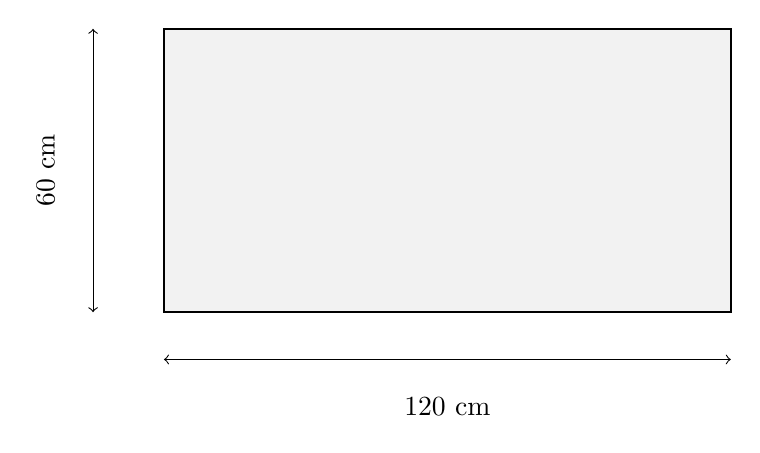
\begin{tikzpicture}[scale=0.06]
    \draw[thick, fill=gray!10] (0,0) rectangle (120,60);
    \draw[<->] (0,-10) -- (120,-10);
    \node at (60,-20) {$120$ cm};
    \draw[<->] (-15,0) -- (-15,60);
    \node[rotate=90] at (-25,30) {$60$ cm};
\end{tikzpicture}
\end{center}

\noindent Work out the perimeter of the bench.
\vspace{4cm}
\begin{flushright}
    \answerunit{cm}{2}
\end{flushright}
\end{question}
